\onecolumn
\thispagestyle{empty}
\newgeometry{top=2.5cm, left=2.5cm, right=3.9cm, bottom=1cm}
 
\begin{wrapfigure}{l}{0.4\columnwidth}
\includegraphics[width=0.4\columnwidth]{cover/monads_good_face}
\vspace{-2.0\baselineskip}
\end{wrapfigure}

%\noindent
\small
This book  is an advanced tutorial
on functional programming in System F$\omega$ using Dhall.

The book's topics include an overview of Dhall's type system;
techniques for numerical calculations in Dhall;
techniques for encoding recursive types and code in System F$\omega$ via the Church encoding;
implementation of various combinators and typeclass derivation for functors, monads, and other
typeclasses;
and some basic applications of dependent types.

The book shows many code examples that have been validated by the Dhall interpreter.

In an appendix, the book shows proofs of some properties of the Church encoding and existential types.

The author received a Ph.D.~in theoretical physics. After a career in academic research, he works as a software engineer.


%\vspace{3.0cm}\hspace*{\fill}\colorbox{white}{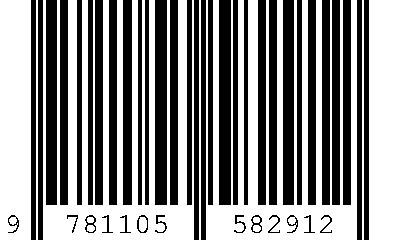
\includegraphics[scale=1.0,width=50.8mm,height=30.5mm]{cover/barcode}}
